\section{Userland security measures}

\subsection{Access Control paradigms: MAC/DAC}

\begin{frame}
	\frametitle{Access control in computer security}
	\begin{itemize}
		\item Access control defines relations between two groups of entities:
			\begin{itemize}
				\item Subjects: entities who can perform an action
				\item Objects: resources that need to be controlled
			\end{itemize}
		\item Access control makes sure only legitimate \emph{subjects} can access
			an \emph{object}
		\item Most systems use one of the following paradigms:
			\begin{itemize}
				\item Discretionary access control (DAC), the most widespread on
					general purpose systems
				\item Mandatory access control (MAC), on systems needing a more
					fine-grained access control
			\end{itemize}
	\end{itemize}
\end{frame}

\begin{frame}
	\frametitle{Discretionary access control}
	\begin{itemize}
		\item Access control is determined by the object owner
			\begin{itemize}
				\item Each object has an owner, e.g.\ the object creator.
				\item The owner assigns permissions to the object, for himself and
					others.
			\end{itemize}
		\item Typical access model:
			\begin{itemize}
				\item Access control list (ACL) based: subjects appear in an
					authorization list linked with the object
				\item Capability based: subjects hold a \emph{capability} that allows to
					manipulate an object
			\end{itemize}
	\end{itemize}
  \begin{center}
		\includegraphics[width=.6\textwidth]{slides/security-userland/dac.pdf}
  \end{center}
\end{frame}

\begin{frame}[fragile]
	\frametitle{POSIX permissions}
	\begin{itemize}
		\item POSIX permission is a typical example of a DAC based on ACL
		\item UNIX philosophy: everything is a file, so each object is represented
			by a file, including devices.
		\item Files metadata include:
			\begin{itemize}
				\item Owning user and owning group
				\item Permissions for each classes: owning user, owning group and others
					\begin{itemize}
						\item Read: grants the ability to read file content
						\item Write: grants the ability to write file content
						\item Execute: grants the ability to execute a file, or read
							metadata of child files when applied on a folder.
					\end{itemize}
				\item Additional permission bits, such as \texttt{setuid} or
					\texttt{setgid}
			\end{itemize}
	\end{itemize}
	\begin{block}{}
		{\tiny
		\begin{verbatim}
$ ls -l /run/
drwxr-xr-x  2 root              root         60 Jan 22 15:51 blkid
-rw-r--r--  1 root              root          5 Jan 22 15:51 blkmapd.pid
drwxr-xr-x  3 root              lp          100 Feb  6 10:26 cups
-rw-r--r--  1 statd             nogroup       5 Jan 22 15:52 rpc.statd.pid
-rw-------  1 root              root          5 Jan 22 15:52 sm-notify.pid
\end{verbatim}
		}
	\end{block}
\end{frame}

\begin{frame}
	\frametitle{Mandatory access control}
	\begin{itemize}
		\item Access control is determined by rules
		\item Rules are controlled by the system administrator
		\item Every time a subject tries to access an object, the operating system
			looks for a corresponding rule
		\item Objects can be accessed only if an existing rule allows this access
		\item Allows to enforce better rules, but more complex to maintain than DAC
		\item Three main implementations for Linux:
			\begin{itemize}
				\item SELinux
				\item AppArmor
				\item TOMOYO Linux
			\end{itemize}
	\end{itemize}
  \begin{flushright}
		\vspace{-1.7cm}
		\includegraphics[width=.6\textwidth]{slides/security-userland/mac.pdf}
  \end{flushright}
\end{frame}

\subsection{Linux capabilities: usage and examples}

\begin{frame}
	\frametitle{Capability based security}
	\begin{itemize}
		\item Theoretical concepts:
			\begin{itemize}
				\item Subjects have capabilities: unforgeable tokens of authority
				\item Capabilities control if and how the subject can manipulate a given object
				\item A given capability specifies access right on a given object.
				\item Completely removes the need of ACL
				\item Examples:
					\begin{itemize}
						\item Subject \emph{user1} can read object \emph{/etc/motd}
						\item Subject \emph{user2} can listen on \emph{TCP port 22} object.
					\end{itemize}
			\end{itemize}
		\item POSIX standard comes with a capabilities specification, differing on
			various points:
			\begin{itemize}
				\item Capabilities are not associated with objects
				\item Capabilities are used in complement of ACL
				\item Examples:
					\begin{itemize}
						\item \emph{CAP\_NET\_BIND\_SERVICE} allows to listen on any privileged
							ports.
					\end{itemize}
			\end{itemize}
	\end{itemize}
\end{frame}


\begin{frame}
	\frametitle{Linux capabilities}
	\begin{itemize}
		\item Capabilities are a per-thread attribute, allowing to gain privileges
			traditionally associated with superuser
		\item Fully integrated since Linux 2.6.24
		\item Capabilities can be independently enabled and disabled
		\item Capabilities can be attached to executable files, pre-setting runtime
			capabilities
		\item Threads may voluntarily enable or disable a capability they are
			permitted to use, allowing to only use them in code paths needing it
		\item Threads may voluntarily preserve capabilities while executing another
			executable (\texttt{execve()}).
	\end{itemize}
\end{frame}

\begin{frame}
	\frametitle{Linux capability examples}
	All capabilities are documented in the
	\href{https://manned.org/capabilities.7}{capabilities(7)} manpage
	\begin{itemize}
		\item
			\href{https://elixir.bootlin.com/linux/v6.19/source/include/uapi/linux/capability.h\#L148}{\texttt{CAP\_KILL}}:
			Bypass permission checks for sending signals
		\item
			\href{https://elixir.bootlin.com/linux/v6.19/source/include/uapi/linux/capability.h\#L205}{\texttt{CAP\_NET\_ADMIN}}:
			Perform various network-related operations
			\begin{itemize}
				\item interface configuration, firewalling, routes, TOS, promiscuous
					mode, multicasting\ldots
			\end{itemize}
		\item
			\href{https://elixir.bootlin.com/linux/v6.19/source/include/uapi/linux/capability.h\#L185}{\texttt{CAP\_NET\_BIND\_SERVICE}}:
			Bind a socket to Internet domain
			privileged ports (port numbers less than 1024).
		\item
			\href{https://elixir.bootlin.com/linux/v6.19/source/include/uapi/linux/capability.h\#L211}{\texttt{CAP\_NET\_RAW}}:
			Use RAW and PACKET sockets
		\item
			\href{https://elixir.bootlin.com/linux/v6.19/source/include/uapi/linux/capability.h\#L154}{\texttt{CAP\_SETGID}},
			\href{https://elixir.bootlin.com/linux/v6.19/source/include/uapi/linux/capability.h\#L159}{\texttt{CAP\_SETUID}}:
			Make arbitrary
			manipulations of process GIDs/UIDs
		\item
			\href{https://elixir.bootlin.com/linux/v6.19/source/include/uapi/linux/capability.h\#L343}{\texttt{CAP\_SETFCAP}}:
			Set arbitrary capabilities on a file.
		\item
			\href{https://elixir.bootlin.com/linux/v6.19/source/include/uapi/linux/capability.h\#L281}{\texttt{CAP\_SYS\_ADMIN}}
			Gives \emph{a lot} of system administration related powers:
			\begin{itemize}
				\item mounts, hostname, privileged log operations, monitoring,
					tracing\ldots
			\end{itemize}
		\item
			\href{https://elixir.bootlin.com/linux/v6.19/source/include/uapi/linux/capability.h\#L285}{\texttt{CAP\_SYS\_BOOT}}:
			Use reboot(2) and kexec\_load(2)
		\item
			\href{https://elixir.bootlin.com/linux/v6.19/source/include/uapi/linux/capability.h\#L224}{\texttt{CAP\_SYS\_MODULE}}:
			Load and unload kernel modules
		\item
			\href{https://elixir.bootlin.com/linux/v6.19/source/include/uapi/linux/capability.h\#L296}{\texttt{CAP\_SYS\_NICE}}:
			Lower the process nice value and change the
			nice value for arbitrary processes, set real-time scheduling policies, set
			CPU affinity\ldots
		\item \ldots
	\end{itemize}
\end{frame}

\begin{frame}
	\frametitle{Thread capability sets}
	\begin{itemize}
		\item Each thread has 5 different capability sets:
			\begin{itemize}
				\item Controlling capabilities a thread is allowed to use:
					\begin{itemize}
						\item Permitted: limits capabilities that might be in \emph{Effective}
							and \emph{Inheritable} sets.\\
							Thread can drop but never add capabilities to this set, except while using
							\texttt{execve()} on a file granting capabilities or with the set-uid bit.
					\end{itemize}
				\item Controlling capabilities effective at the moment:
					\begin{itemize}
						\item Effective: used by the kernel to perform permission checks for the
							thread
					\end{itemize}
				\item Controlling capabilities present while executing a new program:
					\begin{itemize}
						\item Inheritable: capabilities preserved across \texttt{execve()} on
							privileged process
						\item Ambient: capabilities that are preserved across an \texttt{execve()}
							of a program that is not privileged.\\
							Can be used to add capabilities to an unprivileged program
						\item Bounding: capabilities that might be gained on \texttt{execve()}.
							Can be used to limit capabilities that will be acquired from file
							capability sets
					\end{itemize}
			\end{itemize}
	\end{itemize}
\end{frame}

\begin{frame}
	\frametitle{File capability sets}
	\begin{itemize}
		\item Files can be associated with capabilities that will impact thread
			capabilities on \texttt{execve()}:
			\begin{itemize}
				\item Permitted: capabilities automatically permitted to the thread,
					regardless of the thread's inheritable capabilities
				\item Inheritable: capabilities that can be permitted, if they also
					appear in thread \emph{Inheritable} set.
				\item Effective: a single bit determining if \emph{Permitted} set has to
					be copied into the thread \emph{Effective} set.
			\end{itemize}
		\item When executing a program with the \emph{set-user-ID} mode bit set,
			file \emph{Inheritable} and \emph{Permitted} sets are ignored and are
			considered to be all ones.
	\end{itemize}
\end{frame}

\begin{frame}[fragile]
	\frametitle{Manipulating file capability sets}
	\begin{itemize}
		\item \texttt{getcap} can be used to show file capabilities
			\begin{block}{}
				{\tiny
				\begin{verbatim}
$ getcap /usr/lib/x86_64-linux-gnu/gstreamer1.0/gstreamer-1.0/gst-ptp-helper
/usr/lib/x86_64-linux-gnu/gstreamer1.0/gstreamer-1.0/gst-ptp-helper cap_net_bind_service,cap_net_admin,cap_sys_nice=ep
$ getcap -r /usr/bin
/usr/bin/clockdiff cap_net_raw,cap_sys_nice=ep
/usr/bin/dumpcap cap_net_admin,cap_net_raw=eip
\end{verbatim}
}
			\end{block}
			\begin{itemize}
				\item \texttt{gst-ptp-helper} has \texttt{CAP\_NET\_BIND\_SERVICE},
					\texttt{CAP\_NET\_ADMIN} and \texttt{CAP\_SYS\_NICE} in its
					\emph{Permitted} and \emph{Effective} sets
					but not in its \emph{Inheritable} set
				\item \texttt{/usr/bin/clockdiff} has \texttt{CAP\_NET\_RAW} and
					\texttt{CAP\_SYS\_NICE} in its \emph{Permitted} and \emph{Effective} sets
					but not in its \emph{Inheritable} set
				\item \texttt{/usr/bin/dumpcap} has \texttt{CAP\_NET\_ADMIN} and
					\texttt{CAP\_NET\_RAW} in all three sets
			\end{itemize}
		\item \texttt{setcap} can be used to set file capabilities
			\begin{block}{}
				{\tiny
				\begin{verbatim}
# getcap /usr/bin/dumpcap
/usr/bin/dumpcap cap_net_admin,cap_net_raw=eip
# setcap cap_net_admin=eip /usr/bin/dumpcap
# getcap /usr/bin/dumpcap
/usr/bin/dumpcap cap_net_admin=eip
\end{verbatim}
}
			\end{block}
		\item Capabilities syntax is described in
			\href{https://manned.org/cap_from_text.3}{cap\_from\_text(3)} manpage.
	\end{itemize}
\end{frame}

\begin{frame}[fragile,allowframebreaks]
	\frametitle{Manipulating thread capabilities}
	\begin{itemize}
		\item Capabilities can be manipulated through the \texttt{cap\_t} structure.
		\item \texttt{cap\_init()}, \texttt{cap\_dup()} and \texttt{cap\_free()} are
			used to allocate or free a \texttt{cap\_t} instance.
		\item \texttt{cap\_get\_proc()} and \texttt{cap\_set\_proc()} allow to
			retrieve or apply the \texttt{cap\_t} structure corresponding to the
			current thread.
		\item \texttt{cap\_clear()}, \texttt{cap\_set\_flag()} and
			\texttt{cap\_get\_flag()} can be used to manipulate \texttt{cap\_t}
			structure values.
		\item Additional functions and full behaviour are described in
			\href{https://manned.org/cap_get_proc.3}{cap\_get\_proc(3)} and
			\href{https://manned.org/cap_clear.3}{cap\_clear(3)} manpages.
	\end{itemize}
	\begin{block}{}
		{\tiny
    \begin{verbatim}
...
cap_t caps;
const cap_value_t cap_list[2] = {CAP_FOWNER, CAP_SETFCAP};

if (!CAP_IS_SUPPORTED(CAP_SETFCAP))
     /* handle error */

caps = cap_get_proc();
if (caps == NULL)
     /* handle error */;

if (cap_set_flag(caps, CAP_EFFECTIVE, 2, cap_list, CAP_SET) == -1)
     /* handle error */;

if (cap_set_proc(caps) == -1)
     /* handle error */;

if (cap_free(caps) == -1)
     /* handle error */;
...
\end{verbatim}
}
	\end{block}
	\begin{center}
		Example from \href{https://manned.org/cap_get_proc.3}{cap\_get\_proc(3)}
		manpage, adding \texttt{CAP\_FOWNER} and \texttt{CAP\_SETFCAP} effective
		capabilities to the calling thread.
	\end{center}
\end{frame}

\begin{frame}
	\frametitle{setuid and capabilities}
	\begin{itemize}
		\item The \texttt{setuid()} and \texttt{setgid()} syscalls set the effective
			user and group ids
			\begin{itemize}
				\item Can be used by privileged processes to drop privileges or regain
					them later
			\end{itemize}
		\item \texttt{setuid} and \texttt{setgid} flags can be added to file
			permissions to automatically execute them with owner user and group as
			effective IDs
		\item Securebits control the interactions of capabilities and processes with UID 0
			\begin{itemize}
				\item \texttt{SECBIT\_KEEP\_CAPS}: controls if the process retains
					capabilities when switching to non-zero effective UID
				\item \texttt{SECBIT\_NO\_SETUID\_FIXUP}: controls if the kernel should
					adjust capabilities while transitioning between zero and non-zero
					effective UID
				\item \texttt{SECBIT\_NOROOT}: controls if the process is granted
					capabilities while executing a program with the \texttt{setuid} flag
				\item \texttt{SECBIT\_NO\_CAP\_AMBIENT\_RAISE}: controls if the process
					can add new capabilities to the ambient set
				\item Four corresponding \texttt{\_LOCKED} flags exist, preventing from
					ever removing the base flag
			\end{itemize}
	\end{itemize}
\end{frame}

\begin{frame}[fragile]
	\frametitle{Capabilities transformation during execve()}
	\begin{itemize}
		\item The \href{https://manned.org/capabilities.7}{capabilities(7)} manpage
			provides a summary of capabilities transformations:
			\begin{block}{}
				{\small
				\begin{verbatim}
           P'(ambient)     = (file is privileged) ? 0 : P(ambient)
           P'(permitted)   = (P(inheritable) & F(inheritable)) |
                             (F(permitted) & P(bounding)) | P'(ambient)
           P'(effective)   = F(effective) ? P'(permitted) : P'(ambient)
           P'(inheritable) = P(inheritable)    [i.e., unchanged]
           P'(bounding)    = P(bounding)       [i.e., unchanged]

       where:
           P()    denotes the value of a thread capability set before the
                  execve(2)
           P'()   denotes the value of a thread capability set after the
                  execve(2)
           F()    denotes a file capability set
\end{verbatim}
}
			\end{block}
	\end{itemize}
\end{frame}

\subsection{Process isolation: namespaces}

\begin{frame}
	\frametitle{Linux Namespaces}
	\begin{itemize}
		\item A way to partition kernel resources
		\item Different groups of processes will see different resources
		\item In each namespaces, resources appear isolated from the other
			namespaces
		\item One fundamental principle behind software containers
		\item One namespace of each type is created at boot, processes can create or
			join different namespaces during their runtime
		\item Most features were introduced in Linux 3.8 (2013) or before, but some
			new features keep being added
		\item Namespace features are optional: they have to be enabled at kernel
			build time to be used
	\end{itemize}
\end{frame}

\begin{frame}[allowframebreaks]
	\frametitle{Linux Namespaces types}
	\begin{itemize}
		\item Mount namespaces: allowing separation of the filesystem hierarchy.
			Different namespaces will see different mounted filesystems
		\item UTS namespaces: allowing separation of nodename and domainname
		\item IPC namespaces: allowing separation of some IPC resources, such as
			SysV \texttt{shmget()} IPC mechanism
		\item PID namespaces: allowing separation of PIDs.
			Each namespace can reuse the same PID for different processes, e.g.
			PID 1.\\
			The PID will still appear in the host namespace but with a different
			PID
		\item Network namespaces: allowing separation of networking resources.
			Each namespace had a different network configuration: devices, IP
			addresses, routing, firewalling\ldots
		\item User namespaces: allowing to isolate user ids and group ids.
			Ids inside and outside of a namespace can be different, allowing an
			unprivileged user to have the ID 0 inside of the namespace, i.e.\ being
			able to make privileged operations on the namespace resources.
		\item Control group namespaces (introduced in Linux 4.6): allowing cgroup
			hierarchies isolation
		\item Time namespace (introduced in Linux 5.6): allowing namespaces to see a
			different system time
	\end{itemize}
\end{frame}

\begin{frame}
	\frametitle{Namespaces example}
	\begin{itemize}
		\item Namespaces are often combined together
	\end{itemize}
  \begin{center}
		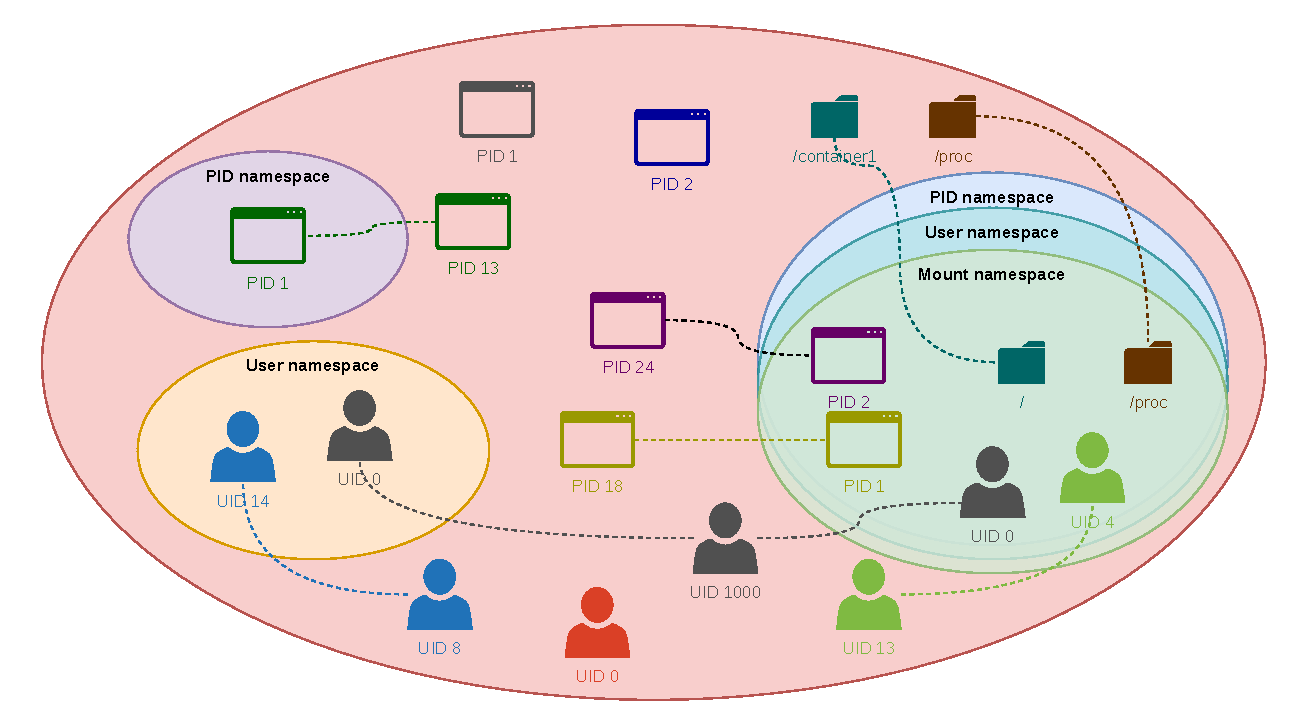
\includegraphics[width=.9\textwidth]{slides/security-userland/namespaces.pdf}
  \end{center}
\end{frame}

\begin{frame}
	\frametitle{Namespace related syscalls (1)}
	\begin{itemize}
		\item Processes can change namespace during their runtime
		\item Various syscalls exist to create or join namespaces
		\item They all take a flag to describe the types of namespaces to manipulate:
			\texttt{CLONE\_NEWNS} (mount namespaces), \texttt{CLONE\_NEWUTS},
			\texttt{CLONE\_NEWIPC}, \texttt{CLONE\_NEWPID}, \texttt{CLONE\_NEWNET},
			\texttt{CLONE\_NEWUSER}, \texttt{CLONE\_NEWCGROUP},
			\texttt{CLONE\_NEWTIME}
		\item Namespaces are deleted automatically when no process is running in
			them and nobody is using a corresponding \texttt{proc/pid/ns/} link file
	\end{itemize}
\end{frame}

\begin{frame}
	\frametitle{Namespace related syscalls (2)}
	\begin{itemize}
		\item \texttt{clone()}:
			\begin{itemize}
				\item Namespace related flags can be specified
				\item The newly created child process will be in different namespace
			\end{itemize}
		\item \texttt{unshare()}:
			\begin{itemize}
				\item Create a new namespace without forking
				\item Also wrapped by the \texttt{unshare} command-line tool
			\end{itemize}
		\item \texttt{setns()}:
			\begin{itemize}
				\item Join an existing namespace
				\item Pointing to a specific namespace:
					\begin{itemize}
						\item First argument: a link file in \texttt{proc/pid/ns/}
						\item Second argument: a single flag describing the namespace type
					\end{itemize}
				\item Pointing to a running process:
					\begin{itemize}
						\item First argument: a PID file descriptor obtained with
							\texttt{pidfd\_open()}
						\item Second argument: a bit mask of flags describing the namespaces
							to join
					\end{itemize}
				\item Also wrapped by the \texttt{nsenter} command-line tool
			\end{itemize}
	\end{itemize}
\end{frame}

\subsection{Process isolation: cgroups}

\begin{frame}
	\frametitle{Linux cgroups}
	\begin{itemize}
		\item Control groups are a way to control resource usages by a group of processes
		\item Resources might include CPU time, RAM, disk\ldots
		\item Such possibilities existed before cgroups, but were enforced per
			process
		\item Control groups allow to:
			\begin{itemize}
				\item Limit resources allocated to a group: CPU time, CPU set, memory,
					number of file descriptors\ldots
				\item Prioritize one group over another one
				\item Measure resource usage, without enforcing any particular limit
			\end{itemize}
		\item cgroup v2 was introduced in Linux kernel 4.5 (2016) with breaking
			changes and a new configuration interface
	\end{itemize}
\end{frame}

\begin{frame}[fragile]
	\frametitle{Cgroup interface: creating cgroups}
	\begin{itemize}
		\item cgroups are configured through a virtual filesystem, generally mounted
			on \texttt{/sys/fs/cgroup}
		\item A new cgroup can be created by creating a new folder in
			\texttt{/sys/fs/cgroup} or an already existing subfolder
			\begin{block}{}
				{\tiny
				\begin{verbatim}
mkdir /sys/fs/cgroup/mygroup
\end{verbatim}
}
			\end{block}
		\item Processes can be assigned to a particular cgroup by writing their PID
			to the \texttt{cgroup.procs} file:
			\begin{block}{}
				{\tiny
				\begin{verbatim}
echo 1234 > /sys/fs/cgroup/mygroup/cgroup.procs
\end{verbatim}
}
			\end{block}
		\item cgroups with no associated processes can be removed by removing the
			associated folder in \texttt{/sys/fs/cgroup}
			\begin{block}{}
				{\tiny
				\begin{verbatim}
rmdir /sys/fs/cgroup/mygroup
\end{verbatim}
}
			\end{block}
	\end{itemize}
\end{frame}

\begin{frame}[fragile,allowframebreaks]
	\frametitle{Cgroup interfaces: controllers}
	\begin{itemize}
		\item Enforcing limits or accessing statistics of a group can be done using
			files of the associated folder in \texttt{/sys/fs/cgroup}
			\begin{block}{}
				{\tiny
				\begin{verbatim}
cat /sys/fs/cgroup/mygroup/memory.current
45056
echo 10000 > /sys/fs/cgroup/mygroup/memory.max
\end{verbatim}
}
			\end{block}
		\item List of all supported controllers can be found in kernel
			documentation:
			\href{https://elixir.bootlin.com/linux/v6.18/source/Documentation/admin-guide/cgroup-v2.rst#L1091}{Documentation/admin-guide/cgroup-v2.rst}
		\item A few examples:
			\begin{itemize}
				\item cpu.stat: read-only file of CPU usage statistics
				\item cpu.max: maximum CPU bandwidth limit
				\item memory.current: read-only file of current memory usage
				\item memory.max: memory usage hard limit
				\item io.stat: read-only file of I/O statistics
				\item pids.max: Hard limit of number of processes
				\item cpuset.cpus: CPUs to be used by tasks of this group
			\end{itemize}
		\item Parent cgroups control whether controllers will be present in their
			childs through the \texttt{cgroup.subtree\_control} control file:
			\begin{block}{}
				{\tiny
				\begin{verbatim}
# echo +cpu -memory -pids > /sys/fs/cgroup/mygroup/cgroup.subtree_control
# cat /sys/fs/cgroup/mygroup/cgroup.subtree_control
cpu
# cat /sys/fs/cgroup/mygroup/mysubgroup/cgroup.controllers
cpu
bootlin-mathieu# ls /sys/fs/cgroup/mygroup/mysubgroup/pids* | wc -l
0
\end{verbatim}
}
			\end{block}
		\item Some statistics files will still be present when the controller is
			disabled:
			\begin{block}{}
				{\tiny
				\begin{verbatim}
#ls -l /sys/fs/cgroup/mygroup/mysubgroup/memory.*
/sys/fs/cgroup/mygroup/mysubgroup/memory.pressure
\end{verbatim}
}
			\end{block}
	\end{itemize}
\end{frame}

\begin{frame}
	\frametitle{Cgroups example}
  \begin{center}
		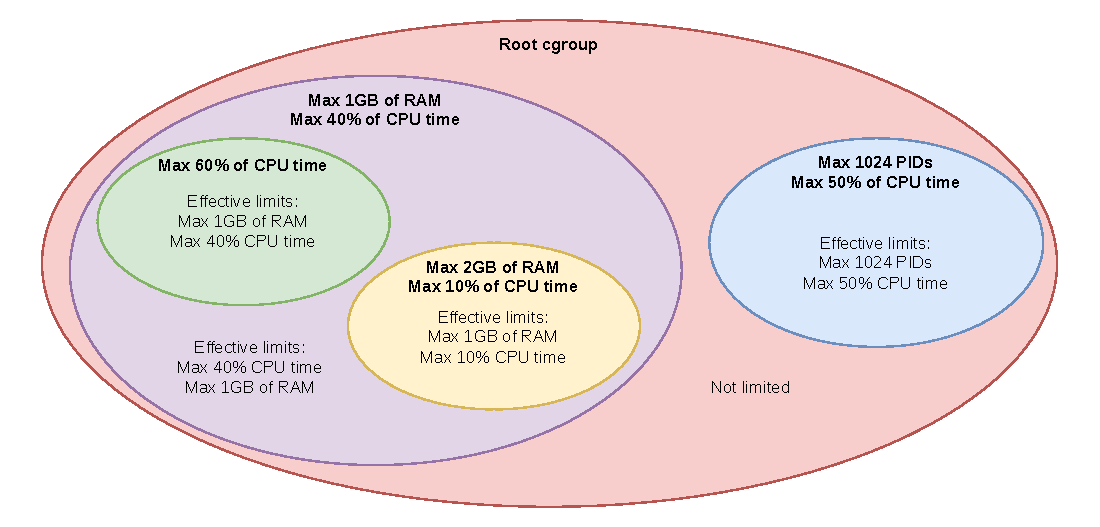
\includegraphics[width=.9\textwidth]{slides/security-userland/cgroups.pdf}
  \end{center}
\end{frame}

\subsection{Process isolation: seccomp}

\begin{frame}[fragile]
	\frametitle{Linux seccomp}
	\begin{itemize}
		\item The linux kernel exposes hundreds of syscalls, but most applications
			only need a few of them
		\item Secure Computing (seccomp) is a kernel feature, allowing to restrict
			the syscalls that a process can use
		\item Processes can voluntarily use the seccomp syscall, restricting
			themselves to use only a few system calls:
			\begin{itemize}
				\item \texttt{read()}
				\item \texttt{write()}
				\item \texttt{exit()}
				\item \texttt{sigreturn()}
			\end{itemize}
		\item If the process later tries to use another syscall, it will be killed
			by the kernel
		\item The seccomp syscall is not wrapped by the glibc: \texttt{syscall()}
			must be used
			\begin{block}{}
				{\tiny
				\begin{verbatim}
syscall(SYS_seccomp, SECCOMP_SET_MODE_STRICT, 0, NULL);
\end{verbatim}
}
			\end{block}
	\end{itemize}
\end{frame}

\begin{frame}[fragile]
	\frametitle{Seccomp filters}
	\begin{itemize}
		\item Some programs might need more than just reading and writing already
			opened files
		\item Seccomp filters were introduced with Linux 3.5
		\item Processes can install a custom BPF program that will filter authorized
			syscalls
			\begin{block}{}
				{\tiny
				\begin{verbatim}
struct sock_fprog prog = { /* BPF program description */ };
syscall(SYS_seccomp, SECCOMP_SET_MODE_FILTER, 0, &prog);
\end{verbatim}
}
			\end{block}
		\item Supported filters are described in
			\href{https://manned.org/seccomp.2}{seccomp(2)} manpage.
		\item This possibility is used by various applications: openSSH, Systemd,
			sudo, Firefox, QEMU\ldots
	\end{itemize}
\end{frame}

\begin{frame}
	\frametitle{Using Seccomp filters}
	\begin{itemize}
		\item Some care must be used when selecting syscalls to filter:
			\begin{itemize}
				\item Most syscalls are abstracted by the libc wrappers: the underlying
					syscall might be different than expected
				\item The same wrapper might used different syscalls on different
					architectures or different libc versions
			\end{itemize}
		\item Additionally, writing BPF code can be tricky
		\item The \emph{libseccomp} library provides a higher level abstraction
			\begin{itemize}
				\item Easier to use
				\item Function based filtering
				\item Platform independent
			\end{itemize}
	\end{itemize}
\end{frame}

\begin{frame}
	\frametitle{Going further on process isolation}
	\begin{itemize}
		\item Namespaces:
			\begin{itemize}
				\item A namespaces article series:
					\url{https://lwn.net/Articles/531114/}
			\end{itemize}
		\item Control groups:
			\begin{itemize}
				\item A control groups article series:
					\url{https://lwn.net/Articles/604609/}
			\end{itemize}
		\item seccomp:
			\begin{itemize}
				\item A seccomp overview: \url{https://lwn.net/Articles/656307/}
				\item About seccomp caveats: \url{https://lwn.net/Articles/738694/}
			\end{itemize}
	\end{itemize}
\end{frame}

\subsection{Linux Security Modules: SELinux}

\begin{frame}
	\frametitle{Security-Enhanced Linux (SELinux)}
	\begin{itemize}
		\item Originally developed by the National Security Agency of the United
			States
		\item Part of mainline Linux since 2.6.0 in 2003
		\item Based on the Linux Security Module (LSM) framework of the kernel
		\item Introduces mandatory access control for userspace components
		\item Additional access control: traditional access control list mechanism
			is still present
		\item SELinux can be used to precisely control which activities a system
			allows each user, process, and daemon
		\item Provided by all major distributions, Yocto and Buildroot
		\item Used on all Android devices
	\end{itemize}
\end{frame}

\begin{frame}[fragile]
	\frametitle{SELinux context}
	\begin{itemize}
		\item Each object (files, users, processes) has a context composed by 3 or 4
			fields:
			\begin{itemize}
				\item user
					\begin{itemize}
						\item An identifier, different from POSIX user
						\item Determines which roles can be used
							\begin{onlyenv}<1>
							\item Each POSIX user is mapped to only one SELinux user
							\item SELinux users can be shared among several POSIX users
							\item Generally used to represent a class of users
							\item E.g. \texttt{user\_u}, \texttt{staff\_u}, \texttt{sysadm\_u}
							\item Mapping between system users and SELinux users can be shown
								with \texttt{semanage login}:
								\begin{block}{}
									{\tiny
									\begin{verbatim}
# semanage login -l

Login Name           SELinux User         MLS/MCS Range        Service

__default__          unconfined_u         s0-s0:c0.c1023       *
root                 unconfined_u         s0-s0:c0.c1023       *
sddm                 xdm                  s0-s0                *
\end{verbatim}
}
								\end{block}
							\end{onlyenv}
					\end{itemize}
					\pause%
				\item role
					\begin{itemize}
						\item Determines what domains can be accessed
						\item Each SELinux user can play a fixed set of roles
							\begin{onlyenv}<2>
							\item E.g. \texttt{system\_r}, \texttt{staff\_r}
							\item List of possible roles for a user can be seen with
								\texttt{seinfo}:
								\begin{block}{}
									{\tiny
									\begin{verbatim}
# seinfo -uunconfined_u -x

Users: 1
    user unconfined_u roles { system_r unconfined_r } level s0 range s0 - s0:c0.c1023;
\end{verbatim}
}
								\end{block}
							\end{onlyenv}
					\end{itemize}
					\pause%
				\item domain or type
					\begin{itemize}
						\item Defines the security context
						\item Most SELinux rules will rely on it
							\begin{onlyenv}<3>
							\item E.g. \texttt{bin\_t}, \texttt{httpd\_t},
								\texttt{my\_application\_t}
							\item List of types for a given role can be seen with
								\texttt{seinfo}
								\begin{block}{}
									{\tiny
									\begin{verbatim}
# seinfo -rstaff_r -x

Roles: 1
   role staff_r types { auditadm_screen_t bluetooth_helper_t chfn_t chkpwd_t
   chromium_naclhelper_t chromium_renderer_t chromium_sandbox_t chromium_t
   container_engine_t container_kvm_t container_t crio_t ddclient_t dirmngr_t
   dockerc_user_t dockerd_t dockerd_user_t evolution_alarm_t evolution_exchange_t
   evolution_server_t evolution_t evolution_webcal_t exim_t games_t gconfd_t gpg_agent_t
    ...
   };
\end{verbatim}
}
								\end{block}
							\end{onlyenv}
					\end{itemize}
					\pause%
				\item range (optional)
					\begin{itemize}
						\item Sometimes referred as \emph{security level}
						\item Can be used as part of \emph{Multi-level security} or
							\emph{Multi-category security}
					\end{itemize}
				\item This context is generally represented as a single string:
					\begin{itemize}
						\item \texttt{user:role:type[:range]}
					\end{itemize}
			\end{itemize}
	\end{itemize}
\end{frame}

\begin{frame}
	\frametitle{Multi-Level and Multi-Category Security}
	\begin{itemize}
		\item Multi-Level Security (MLS)
			\begin{itemize}
				\item Allows a hierarchical structure representing different level of
					sensitivity
				\item Levels can be used to represent data classification
					\begin{itemize}
						\item Unclassified, Restricted, Confidential, Secret\ldots
					\end{itemize}
			\end{itemize}
		\item Multi-Category Security (MCS)
			\begin{itemize}
				\item Allows to compartment data with different categories
				\item Categories can be used to represent different departments
			\end{itemize}
		\item SELinux allows to mix both levels and categories
	\end{itemize}
\end{frame}

\begin{frame}
	\frametitle{SELinux Multi-Level and Multi-Category Security}
	\begin{itemize}
		\item Context \emph{range} can be composed by two parts:
			\begin{itemize}
				\item The sensitivity level, as an integer
					\begin{itemize}
						\item Order is defined by the \emph{dominance}, s0 is generally the
							lowest
						\item For MCS, only one level is used: typically s0
					\end{itemize}
				\item Optionally, the category set, as integers
			\end{itemize}
		\item Ranges are represented as strings
			\begin{itemize}
				\item \texttt{s0}: sensitivity level 0
				\item \texttt{s1:c4,c7}: sensitivity level 1, categories 4 and 7
			\end{itemize}
		\item Domains will be affected a clearance
			\begin{itemize}
				\item Determines which level and categories can be accessed
				\item \texttt{s2:c1.c4,c7}: sensitivity level 2, categories 1 to 4 and 7
				\item \emph{dominance} determinates other allowed security levels
			\end{itemize}
	\end{itemize}
\end{frame}

\begin{frame}[fragile]
	\frametitle{SELinux file context}
	\begin{itemize}
		\item On creation, files and directories will by default inherit the context
			of parent folder
		\item \texttt{ls -Z} can be used to show file context:
			\begin{block}{}
				{\tiny
				\begin{verbatim}
# ls -lZ /
lrwxrwxrwx.   1 root root system_u:object_r:bin_t:s0                   7 Feb 19 08:09 bin -> usr/bin
drwxr-xr-x.   3 root root system_u:object_r:boot_t:s0               4096 Feb 19 08:11 boot
drwxr-xr-x.  19 root root system_u:object_r:device_t:s0             3300 Feb 19 08:29 dev
drwxr-xr-x.  78 root root system_u:object_r:etc_t:s0                4096 Feb 19 08:28 etc
drwxr-xr-x.   3 root root system_u:object_r:home_root_t:s0          4096 Feb 19 08:11 home
...
\end{verbatim}
}
			\end{block}
		\item \texttt{chcon} can be used to change file context:
			\begin{block}{}
				{\tiny
				\begin{verbatim}
# ls -lZ hello.sh
-rwxr-xr-x. 1 root root unconfined_u:object_r:user_home_t:s0 23 Feb 19 08:29 hello.sh
# chcon system_u:object_r:bin_t:s0 hello.sh
# ls -lZ hello.sh
-rwxr-xr-x. 1 root root system_u:object_r:bin_t:s0 23 Feb 19 08:29 hello.sh
\end{verbatim}
}
			\end{block}
		\item \texttt{restorecon} can be used to set file context to policy default
			values
	\end{itemize}
\end{frame}

\begin{frame}[fragile]
	\frametitle{SELinux process context}
	\begin{itemize}
		\item On creation, processes will by default inherit the context of parent
			process
		\item \texttt{id -Z} can be used to show own context in a shell:
			\begin{block}{}
				{\tiny
				\begin{verbatim}
# id -Z
unconfined_u:unconfined_r:unconfined_t:s0-s0:c0.c1023
\end{verbatim}
}
			\end{block}
		\item \texttt{ps -Z} can be used to show processes contexts:
			\begin{block}{}
				{\tiny
				\begin{verbatim}
# ps -Z
LABEL                               PID TTY          TIME CMD
unconfined_u:unconfined_r:unconfined_t:s0-s0:c0.c1023 738 pts/0 00:00:00 bash
unconfined_u:unconfined_r:unconfined_t:s0-s0:c0.c1023 1608 pts/0 00:00:00 ps
\end{verbatim}
}
			\end{block}
		\item \texttt{runcon} can be used to start a process with a different
			context:
			\begin{itemize}
				\item The transition must be allowed by SELinux policy rules
					\begin{block}{}
						{\tiny
						\begin{verbatim}
# id -Z
unconfined_u:unconfined_r:unconfined_t:s0-s0:c0.c1023
# runcon -r system_r bash
# id -Z
unconfined_u:system_r:unconfined_t:s0-s0:c0.c1023
\end{verbatim}
}
					\end{block}
			\end{itemize}
	\end{itemize}
\end{frame}

\begin{frame}[fragile]
	\frametitle{SELinux modes}
	\begin{itemize}
		\item SELinux can be used in two different modes
			\begin{itemize}
				\item Permissive: rules are not enforced, but all violations are logged
					\begin{itemize}
						\item Can be useful during the configuration phase to ensure
							all needed rules have been set.
						\item The \texttt{audit2allow} tool can then be used to generate
							some rules based on this log
					\end{itemize}
				\item Enforcing: rules are strictly enforced
			\end{itemize}
		\item Mode can be configured in \texttt{/etc/selinux/config} or with
			\texttt{setenforce}
		\item Additionally, SELinux can be completely disabled
		\item Active mode can be seen with \texttt{sestatus}
			\begin{block}{}
				{\tiny
				\begin{verbatim}
# sestatus
SELinux status:                 enabled
SELinuxfs mount:                /sys/fs/selinux
SELinux root directory:         /etc/selinux
Loaded policy name:             default
Current mode:                   permissive
...
\end{verbatim}
}
			\end{block}
	\end{itemize}
\end{frame}

\begin{frame}[fragile]
	\frametitle{SELinux policies}
	\begin{itemize}
		\item Policies will describe what is permitted on the system
			\begin{itemize}
				\item By default, everything is forbidden
				\item Rules will allow processes to use objects, based on the context of
					both the source and the target
			\end{itemize}
		\item Policies can be dynamically loaded during runtime
		\item Policies will have to adapt to system needs:
			\begin{itemize}
				\item They can only isolate a few processes
				\item They can implement a full multi-level security system
				\item Or implement anything in-between
			\end{itemize}
	\end{itemize}
\end{frame}

\begin{frame}
	\frametitle{SELinux rules}
	\begin{itemize}
		\item SELinux rules are based on a \emph{access vector} describing the
			access, composed by:
			\begin{itemize}
				\item The source context
				\item The target context
				\item The class of the target
					\begin{itemize}
						\item Describes the type of the resource
						\item E.g. \texttt{file}, \texttt{socket}, \texttt{process},
							\texttt{dbus}
					\end{itemize}
				\item the permission or activity
					\begin{itemize}
						\item Describes the action the access tries to make
						\item Possible values depend on the class
						\item E.g. \texttt{create}, \texttt{read}, \texttt{write},
							\texttt{execute}, \texttt{bind}, \texttt{connect}
					\end{itemize}
			\end{itemize}
	\end{itemize}
\end{frame}

\begin{frame}[fragile]
	\frametitle{SELinux rules examples}
	\begin{itemize}
		\item Most SELinux rules rely on the type, but other context fields can also
			be used
		\item The most common rule is \texttt{allow}, allowing a specific access
			\begin{block}{}
				{\tiny
				\begin{verbatim}
allow user_t lib_t : file { execute };
\end{verbatim}
}
			\end{block}
			\begin{itemize}
				\item Allows processes from \texttt{user\_t} domain
				\item To \texttt{execute} \texttt{files}
				\item Of the \texttt{lib\_t} type
			\end{itemize}
		\item Other types of rules exist, such as \texttt{type\_transition},
			allowing process transition to a different context:
			\begin{block}{}
				{\tiny
				\begin{verbatim}
type_transition init_t initrc_exec_t : process initrc_t;
\end{verbatim}
}
			\end{block}
			\begin{itemize}
				\item Processes running in \texttt{init\_t} domain
				\item Executing a file with \texttt{initrc\_exec\_t} type
				\item Shall transition to the \texttt{initrc\_t} domain
			\end{itemize}
	\end{itemize}
\end{frame}

\begin{frame}[fragile]
	\frametitle{Listing SELinux rules}
	\begin{itemize}
		\item The \texttt{sesearch} command can be used to query rules present on
			the system
			\begin{itemize}
				\item Filters can be added on the type of rules:
					\begin{itemize}
						\item \texttt{--allow}
						\item \texttt{--role\_transition}
						\item \ldots
					\end{itemize}
				\item Filters can also be added on context fields:
					\begin{itemize}
						\item \texttt{-s}: source context
						\item \texttt{-t}: target context
						\item \texttt{-c}: object class
						\item \ldots
					\end{itemize}
			\end{itemize}
			\begin{block}{}
				{\tiny
				\begin{verbatim}
# sesearch --allow --source wireshark_t --target proc_net_t
allow wireshark_t proc_net_t:dir { getattr ioctl lock open read search };
allow wireshark_t proc_net_t:file { getattr ioctl lock open read };
allow wireshark_t proc_net_t:lnk_file { getattr read };
\end{verbatim}
}
			\end{block}
	\end{itemize}
\end{frame}

\begin{frame}[fragile]
	\frametitle{SELinux policy modules}
	\begin{itemize}
		\item SELinux comes with the concept of modules, providing rules
		\item Policy modules can be dynamically loaded or unloaded with
			\texttt{semodule}
			\begin{itemize}
				\item \texttt{--list-modules}
				\item \texttt{--enable}
				\item \texttt{--disable}
			\end{itemize}
			\begin{block}{}
				{\tiny
				\begin{verbatim}
# semodule --list-modules | head -5
accountsd
acct
afs
aide
alsa
# semodule --disable alsa
libsemanage.add_user: user sddm not in password file
root@setest:~# semodule --list-modules | grep alsa
\end{verbatim}
}
			\end{block}
		\item Generic policies might be provided by projects, distributions or the
			\href{https://github.com/SELinuxProject/refpolicy}{SELinux refpolicy
			project}
	\end{itemize}
\end{frame}

\begin{frame}
	\frametitle{Creating SELinux policies}
	\begin{itemize}
		\item You will sometimes need to write your own policies
			\begin{itemize}
				\item For your own custom context
				\item For a project you are maintaining
			\end{itemize}
		\item Typical policy modules will consist of:
			\begin{itemize}
				\item A \texttt{.te} file containing policy rules for your application,
					such as \texttt{allow} or transition rules
				\item A \texttt{.if} file defining the interfaces: policy macros used by
					other policy modules to interact with this policy
				\item A \texttt{.fc} file defining application security contexts:
					instructions for labeling files related to the application
			\end{itemize}
	\end{itemize}
\end{frame}

\begin{frame}[fragile]
	\frametitle{Creating SELinux policies: sepolicy generate}
	\begin{itemize}
		\item The \texttt{sepolicy generate} command can be used to create module
			template files
		\item SELinux can be generated from the above files with
			\texttt{checkmodule} and \texttt{semodule\_package} or more easily with
			some helper script
			\begin{block}{}
				{\tiny
				\begin{verbatim}
# mkdir myapp && cd myapp
# sepolicy generate --init -n myapp /bin/myapp
Failed to retrieve rpm info for selinux-policy
Created the following files:
/root/myapp/myapp.te # Type Enforcement file
/root/myapp/myapp.if # Interface file
/root/myapp/myapp.fc # File Contexts file
/root/myapp/myapp_selinux.spec # Spec file
/root/myapp/myapp.sh # Setup Script
# ... Define your custom rules ...
# ./myapp.sh
# semodule -l | grep myapp
myapp
\end{verbatim}
}
			\end{block}
		\item In most cases, audit2allow can help you to define those rules
	\end{itemize}
\end{frame}

\subsection{Linux Security Modules: AppArmor}

\begin{frame}
	\frametitle{AppArmor}
	\begin{itemize}
		\item Developed by Immunix in 1998
		\item Supported by Canonical since 2009
		\item Allows limiting program capabilities with profiles
		\item Provides an alternative to SELinux:
			\begin{itemize}
				\item Allows to introduce MAC in Linux systems
				\item Based on the Linux Security Module (LSM) framework of the kernel
			\end{itemize}
	\end{itemize}
\end{frame}

\begin{frame}
	\frametitle{AppArmor differences with SELinux}
	\begin{itemize}
		\item Files are identified by their path instead of attaching \emph{security
			labels} to inodes
			\begin{itemize}
				\item Creating a hardlink to a restricted file might help to bypass
					restrictions
			\end{itemize}
		\item As no data is stored in file inodes, the configuration is more
			centralized
		\item AppArmor only supports about 20 \emph{Access Modes}:
			\begin{itemize}
				\item SELinux supports hundreds of different permissions, depending on
					the type of object
				\item Basic modes: \texttt{read}, \texttt{write}, \texttt{append}
				\item Execution mode, with various variants
				\item Link files and lock files management
			\end{itemize}
		\item There is no support for multi-level security
		\item Overall, AppArmor tends to provide less advanced features but to be
			also easier to use
	\end{itemize}
\end{frame}

\begin{frame}
	\frametitle{AppArmor profile files}
	\begin{itemize}
		\item AppArmor relies on \emph{Profiles} to describe applications confinement
		\item Simple text files stored in \texttt{/etc/apparmor.d}, one file per
			binary
			\begin{itemize}
				\item Files are named to reflect binary path, \texttt{/} being replaced
					by \texttt{.}
				\item E.g. \texttt{/etc/apparmor.d/bin.ping} for \texttt{/bin/ping}
			\end{itemize}
		\item Profiles will contain rules:
			\begin{itemize}
				\item Paths of files that can be accessed
				\item Capabilities that can be used
			\end{itemize}
		\item \texttt{aa-genprof} can be used to automatically create a new profile
			\begin{itemize}
				\item Target application is launched, all actions are logged
				\item The user is then prompted for actions that need to be allowed by
					profile rules
				\item Similarly, \texttt{aa-logprof} can be used to interactively add
					rules from audit logs
			\end{itemize}
	\end{itemize}
\end{frame}

\begin{frame}[fragile]
	\frametitle{AppArmor profile example}
	\begin{itemize}
		\item \texttt{/etc/apparmor.d/bin.ping} content:
			\begin{block}{}
				{\tiny
				\begin{verbatim}
abi <abi/4.0>,

include <tunables/global>
profile ping /{usr/,}bin/{,iputils-}ping flags=(complain) {
  include <abstractions/base>
  include <abstractions/consoles>
  include <abstractions/nameservice>

  capability net_raw,
  capability setuid,
  network inet raw,
  network inet6 raw,

  /{,usr/}bin/{,iputils-}ping mixr,
  /etc/modules.conf r,
  @{PROC}/sys/net/ipv6/conf/all/disable_ipv6 r,
}
\end{verbatim}
}
			\end{block}
		\item This profile can be used by \texttt{ping} and \texttt{iputils-ping}
			binaries
		\item Allows to use \texttt{net\_raw} and \texttt{setuid} capabilities
		\item Add m (executable mapping), ix (inherit execute mode) and r (read)
			access modes to the \texttt{ping} binary
		\item Add r (read) access mode to \texttt{/etc/modules.conf} and
			\texttt{/proc/sys/net/ipv6/conf/all/disable\_ipv6} files
	\end{itemize}
\end{frame}

\begin{frame}[fragile]
	\frametitle{AppArmor base commands (1)}
	\begin{itemize}
		\item \texttt{aa-status}
			\begin{itemize}
				\item Shows current AppArmor status
			\begin{block}{}
				{\tiny
				\begin{verbatim}
# aa-status
apparmor module is loaded.
126 profiles are loaded.
6 profiles are in enforce mode.
   /usr/bin/man
   lsb_release
   ...
44 profiles are in complain mode.
   Xorg
   avahi-daemon
   dnsmasq
   ...
\end{verbatim}
}
			\end{block}
			\end{itemize}
		\item \texttt{aa-complain} and \texttt{aa-enforce}
			\begin{itemize}
				\item Either enter complain (audit) or enforce mode for a given profile
			\begin{block}{}
				{\tiny
				\begin{verbatim}
# aa-enforce /bin/ping
\end{verbatim}
}
			\end{block}
			\end{itemize}
	\end{itemize}
\end{frame}

\begin{frame}[fragile]
	\frametitle{AppArmor base commands (2)}
	\begin{itemize}
		\item \texttt{apparmor\_parser}
			\begin{itemize}
				\item Load or reload a profile file
			\end{itemize}
			\begin{block}{}
				{\tiny
				\begin{verbatim}
# apparmor_parser -r /etc/apparmor.d/bin.ping
\end{verbatim}
}
			\end{block}
		\item \texttt{aa-exec}
			\begin{itemize}
				\item Execute a program with non-default profile
			\end{itemize}
			\begin{block}{}
				{\tiny
				\begin{verbatim}
# aa-exec -p unconfined -- ping bootlin.com
\end{verbatim}
}
			\end{block}
	\end{itemize}
\end{frame}

\begin{frame}[fragile]
	\frametitle{AppArmor audit log}
	\begin{itemize}
		\item AppArmor log will list rules violations
			\begin{itemize}
				\item We can test with a modified \emph{ping} profile, with
					\texttt{net\_raw} capability removed
			\end{itemize}
			\begin{block}{}
				{\tiny
				\begin{verbatim}
# aa-enforce /bin/ping
# ping -N name bootlin.com
ping: socktype: SOCK_RAW
ping: socket: Permission denied
# grep success=no /var/log/audit/audit.log  
type=SYSCALL msg=audit(1771853258.629:191): arch=c000003e syscall=41 success=no exit=-13 a0=2 a1=3 a2=1 a3=6 items=0 ppid=849 pid=869
auid=0 uid=0 gid=0 euid=0 suid=0 fsuid=0 egid=0 sgid=0 fsgid=0 tty=pts0 ses=1 comm="ping" exe="/usr/bin/ping" subj=ping
key=(null)ARCH=x86_64 SYSCALL=socket AUID="root" UID="root" GID="root" EUID="root" SUID="root" FSUID="root" EGID="root" SGID="root"
FSGID="root"
\end{verbatim}
}
			\end{block}
	\end{itemize}
\end{frame}

\subsection{Application hardening via systemd}

\begin{frame}
	\frametitle{Systemd}
	\begin{itemize}
		\item Modern \emph{init} system used by almost all Linux
			desktop/server distributions
		\item Provides features such as
			\begin{itemize}
				\item Parallel startup of services, taking into account
					dependencies
				\item Monitoring of services
				\item On-demand startup of services, through \emph{socket activation}
				\item Resource-management of services: CPU limits, memory limits
			\end{itemize}
		\item Configuration based on \emph{unit files}
			\begin{itemize}
				\item Declarative language, instead of shell scripts used in other init
					systems
			\end{itemize}
	\end{itemize}
\end{frame}

\begin{frame}
	\frametitle{Capabilities related settings}
	\begin{itemize}
		\item Systemd execution units allow to specify capabilities related settings
			\begin{itemize}
				\item \texttt{CapabilityBoundingSet=} controls which capabilities should be
					in the process bounding set
				\item \texttt{AmbientCapabilities=} controls which capabilities should be in
					the process ambient set
				\item \texttt{SecureBits=} controls which Securebits should be set
				\item \texttt{NoNewPrivileges=} is a boolean value, controlling if
					\texttt{PR\_SET\_NO\_NEW\_PRIVS} flag should be applied with
					\texttt{prctl()}.  If set, ensure no new privilege is ever gained
					through \texttt{execve()}: effective UID and GID are not affected by
					\texttt{setuid} and \texttt{setgid} bits, capabilities cannot be
					added.
			\end{itemize}
	\end{itemize}
\end{frame}

\begin{frame}
	\frametitle{SELinux and AppArmor control}
	\begin{itemize}
		\item Systemd execution units allow to control SELinux context or AppArmor
			profile
			\begin{itemize}
				\item \texttt{SELinuxContext=} Sets the SELinux security context,
					overriding the default transition. The transition must be allowed by
					the SELinux policy.
				\item \texttt{AppArmorProfile=} Sets the AppArmor profile to use. The
					profile must already be loaded in the kernel.
			\end{itemize}
	\end{itemize}
\end{frame}

\begin{frame}
	\frametitle{Process sandboxing}
	\begin{itemize}
		\item Systemd execution units allow to sandbox processes
			\begin{itemize}
				\item Can be used to limit the system exposure
				\item Sandboxing options relies on various kernel features: seccomp,
					namespaces\ldots
				\item Highly simplifies usage of various security features
			\end{itemize}
		\item All options are described in the \emph{SANDBOXING} section of the
			\href{https://manned.org/systemd.exec.5}{systemd.exec(5)}
			manpage
		\item A good practice is to enable as much as possible of these options
	\end{itemize}
\end{frame}

\begin{frame}
	\frametitle{Process sandboxing examples}
	\begin{itemize}
		\item Data access:
			\begin{itemize}
				\item Some directories can be made inaccessible, read-only, or replaced
					by a temporary empty folder
			\end{itemize}
		\item Device access:
			\begin{itemize}
				\item \texttt{/dev} can be replaced by a folder with only a few pseudo
					devices, such as \texttt{/dev/null} or \texttt{/dev/zero}
				\item A separate network namespace or a completely isolated network can
					be used. Alternatively, communication can be restricted to some socket
					families
			\end{itemize}
		\item System configuration:
			\begin{itemize}
				\item Various parts of \texttt{/proc} can be made read-only
				\item Kernel modules loading can be blocked
				\item Realtime scheduling can be limited
			\end{itemize}
		\item Dedicated namespaces can be used: IPC, PID, UTS, clocks\ldots
	\end{itemize}
\end{frame}

\begin{frame}
	\frametitle{Syscall filtering with Systemd}
	\begin{itemize}
		\item Systemd allows to filter syscalls used by launched process
		\item Relies on \texttt{seccomp} kernel feature
		\item The \texttt{SystemCallFilter=} settings can be used to define the list
			of allowed or forbidden syscalls
		\item As for using seccomp directly, remember getting the correct list of
			syscalls might be tricky
		\item Syscalls are grouped in predefined sets that can be used instead of
			listing them individually:
			\begin{itemize}
				\item \texttt{@basic-io}, system calls for basic I/O: \texttt{read()},
					\texttt{write()} and related calls
				\item \texttt{@mount}, mounting and unmounting of file system:
					\texttt{mount()}, \texttt{chroot()}, and related calls
				\item \texttt{@reboot}, System calls for rebooting and reboot
					preparation: \texttt{reboot()}, \texttt{kexec()}, and related calls
				\item \ldots
			\end{itemize}
	\end{itemize}
\end{frame}

\begin{frame}
	\frametitle{Systemd resource control}
	\begin{itemize}
		\item Systemd allows to limit process resources, relying on Linux cgroups
			\begin{itemize}
				\item Controlling CPU usage: \texttt{CPUAccounting=},
					\texttt{CPUQuota=}, \texttt{AllowedCPUs=}\ldots
				\item Controlling memory usage: \texttt{MemoryAccounting=},
					\texttt{MemoryMin=}, \texttt{MemoryHigh=}, \texttt{MemoryMax=}\ldots
				\item Controlling number of tasks: \texttt{TasksAccounting=},
					\texttt{TasksMax=}
				\item Controlling I/O throughput: \texttt{IOAccounting=},
					\texttt{IOReadBandwidthMax=}, \texttt{IOReadIOPSMax=}\ldots
				\item Controlling network usage: \texttt{IPAccounting=},
					\texttt{SocketBindAllow=}, \texttt{RestrictNetworkInterfaces=}\ldots
			\end{itemize}
		\item All settings are described in
			\href{https://manned.org/systemd.resource-control.5}{systemd.resource-control(5)}
			manpage.
	\end{itemize}
\end{frame}

\begin{frame}[fragile]
	\frametitle{Systemd service example: openvpn@.service}
	\begin{block}{}
		{\tiny
		\begin{verbatim}
[Unit]
Description=OpenVPN connection to %i
...

[Service]
Type=notify
PrivateTmp=true
WorkingDirectory=/etc/openvpn
ExecStart=/usr/sbin/openvpn --daemon ovpn-%i --status /run/openvpn/%i.status 10 --cd /etc/openvpn --config /etc/openvpn/%i.conf
    --writepid /run/openvpn/%i.pid
PIDFile=/run/openvpn/%i.pid
KillMode=process
CapabilityBoundingSet=CAP_IPC_LOCK CAP_NET_ADMIN CAP_NET_BIND_SERVICE CAP_NET_RAW CAP_SETGID CAP_SETUID CAP_SETPCAP CAP_SYS_CHROOT
    CAP_DAC_OVERRIDE CAP_AUDIT_WRITE
TasksMax=10
DeviceAllow=/dev/null rw
DeviceAllow=/dev/net/tun rw
ProtectSystem=true
ProtectHome=true
RestartSec=5s
Restart=on-failure
\end{verbatim}
		}
	\end{block}
\end{frame}

% TODO: talk about RootHash=/RootVerity= ?
